\section{Kanalcodierung}
Ziel: Redundanz hinzufügen

\subsection{Fehlerkorrekturverfahren}
\textbf{Backward Error Correction: } Die Redundanz erlaubt lediglich, Fehler zu erkennen und eine Neuübertragung der Daten anzufordern. \\
\textbf{Forward Error Correction: } Die von der Kanalcodierung hinzugefügte Redundanz reicht, um bei Empfänger Fehler zu korrigieren.

\subsection{Binäre Kanäle}%
Binäre Kanäle können nur die Werte 0 und 1 übertragen. Übertragungsfehler entstehen dadurch, dass ein Bit geflipped wird.

\textbf{$\varepsilon$ ist die Bitfehlerwahrscheinlichkeit (BER Bit Error Ratio)}

\subsubsection{Bitfehlerwahrscheinlichkeit}
Die Bitfehlerwahrscheinlichkeit ε ist eine Eigenschaft des Kanals. \\
Für den symmetrischen Binären Kanal (BSC) gilt:
\begin{enumerate}
    \item Die Fehlerwahrscheinlichkeit ist unabhängig vom Eingangssymbol
    \item Die Wahrscheinlichkeiten $P(y_m|x_n)$ der Übergänge bei gegebenem $x_n$ sind:
\end{enumerate}
\begin{center}
    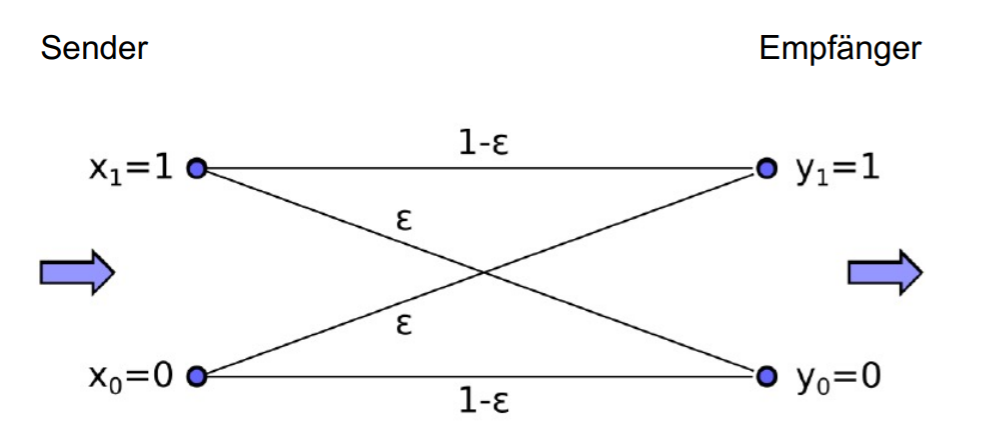
\includegraphics[width=1\linewidth]{images/fehlerwahrscheinlichkeiten.png}
\end{center}
\textbf{Erfolgswahrscheinlichkeit: } $P_{0,N}=\frac{A_N}{A}=(1-\varepsilon)^N$ \\
\textbf{Fehlerwahrscheinlichkeit: } (auf N Datenbits) $1-P_{0,N}=1-(1-\varepsilon)^N$
\begin{center}
    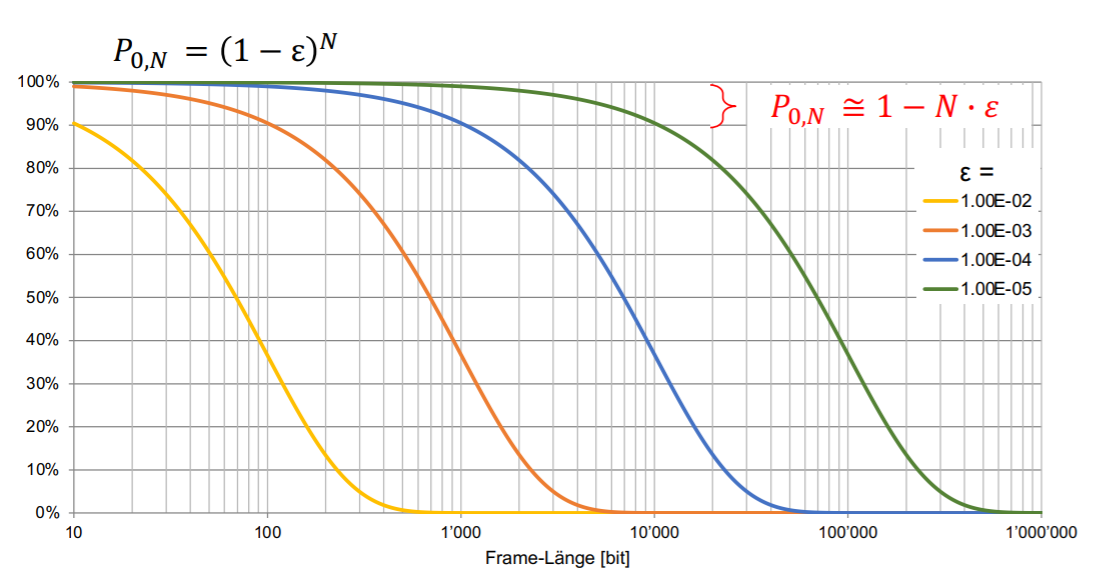
\includegraphics[width=1\linewidth]{images/fehlergraph.png}
\end{center}

\subsubsection{Mehr-Bit-Fehlerwahrscheinlichkeit einer Sequenz}%
Die Wahrscheinlichkeit $P_{F,N}$, dass in einer Sequenz von $N$ Datenbits genau $F$ Bitfehler auftreten, ist:
\[
    P_{F,N} = \binom{N}{F} \cdot \varepsilon^F \cdot (1-\varepsilon)^{N-F}
\]

\begin{center}
    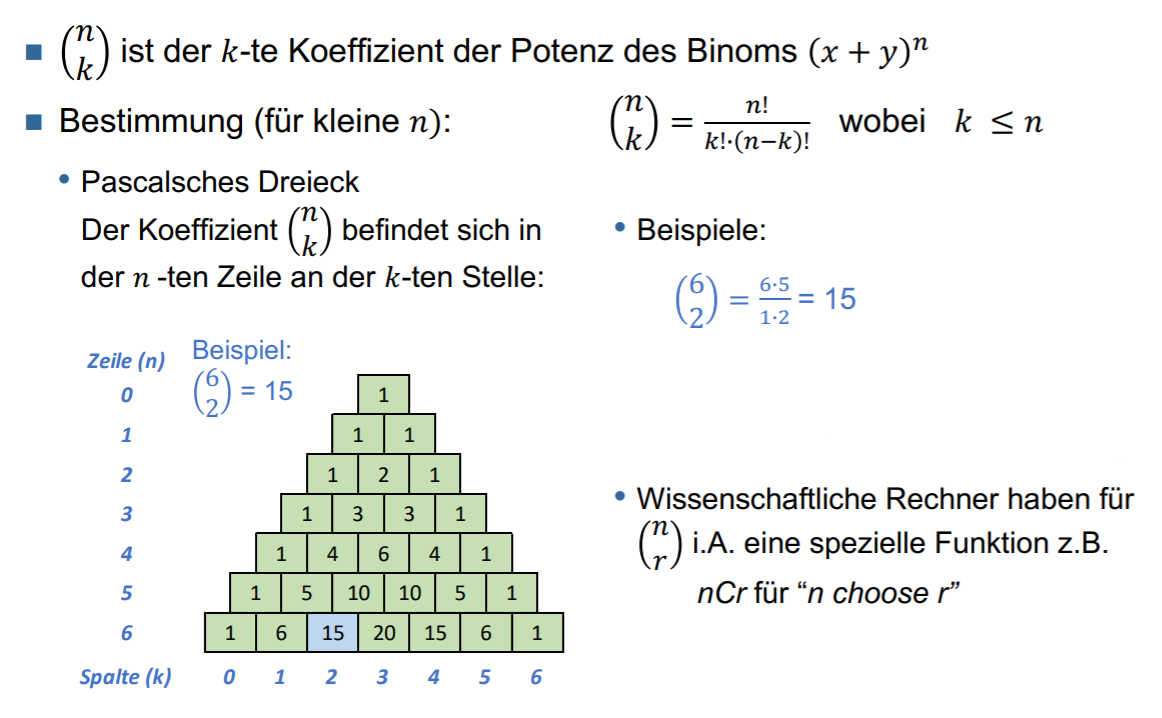
\includegraphics[width=1\linewidth]{images/binominalcoefficient.png}
\end{center}

Für die Wahrscheinlichkeit, dass maximal F Fehler bei einer Übertragung von N Bits auftreten, bilden wir die Summe aller Fälle:
\[
    P_{\leq F, N} = \sum^{F}_{t=0}\binom{N}{t} \cdot \varepsilon^t \cdot (1-\varepsilon)^{N-t}
\]

Restfehlerwahrscheinlichkeit (mehr als F Fehler bei einer Übertragung von N Bits):
\[
    P_{>F,N}=\sum^{N}_{t=F+1}\binom{N}{t} \cdot \varepsilon^t \cdot (1-\varepsilon)^{N-t}
\]

\subsection{Kanalkapazität des BSC}%

Die maximale Kanalkapazität entspricht der Entropie einer binären Quelle: 1bit/Symbol = 1 bit/bit.

\begin{center}
    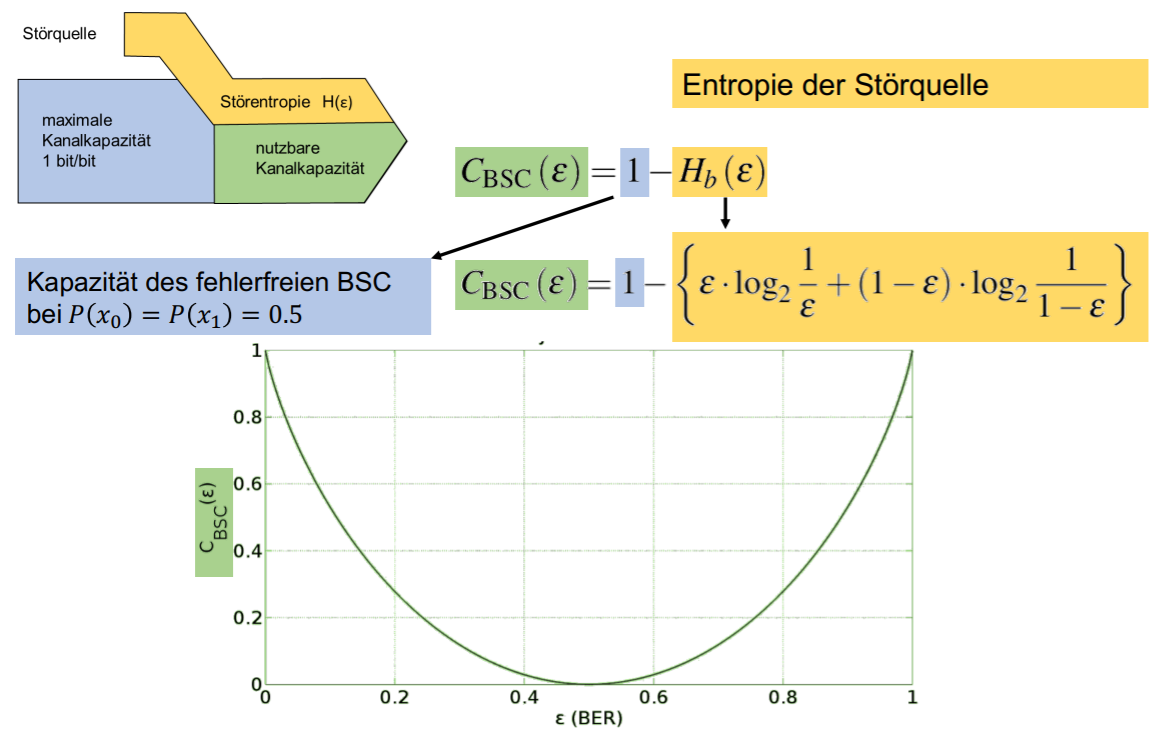
\includegraphics[width=1\linewidth]{images/kanalkapazitaet.png}
\end{center}

\subsubsection{Eingangs- und Ausgangswahrscheinlichkeiten}%

\begin{center}
    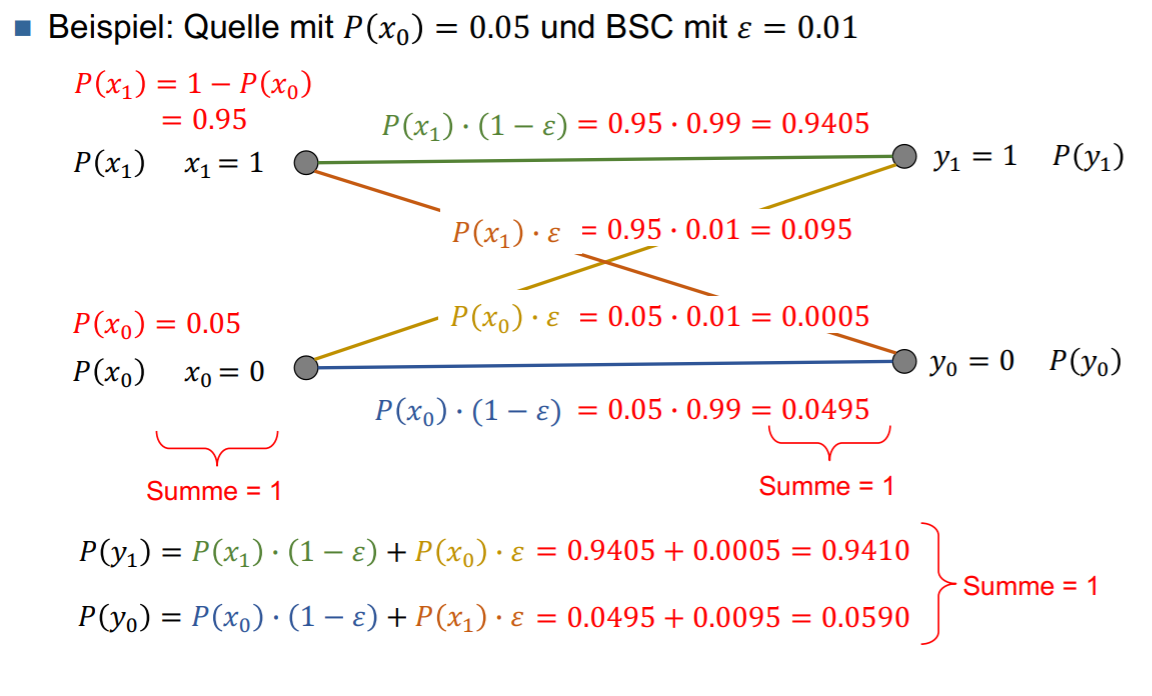
\includegraphics[width=1\linewidth]{images/einauswahrscheinlichkeit.png}
\end{center}

\subsubsection{Entropien eines BSC}%

\begin{center}
    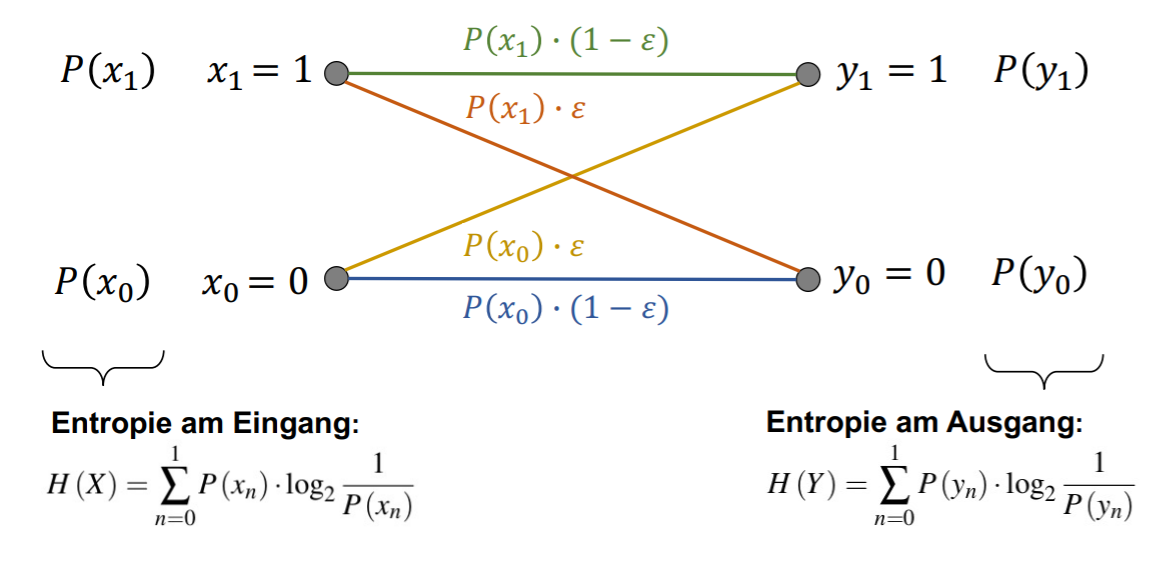
\includegraphics[width=1\linewidth]{images/bscentropy.png}
\end{center}

\subsubsection{Gemeinsame Information}%
Die übertragene Information, die dem Eingang und dem Ausgang gemeinsam ist, kan trotz Fehlern übertragen werden. Sind H(Y) und H(ε) bekannt, folgt für die gemeinsame Information I(X,Y): \textbf{$I(X,Y) = H(Y) - H(\varepsilon) [bit/bit]$}

\subsection{Hamming Distanz}%
\label{sub:hamming_distanz}

Hamming-Distanz ist die Anzahl der wechselnden Bits von einem gültigen Code zum nächsten gültigen Code. Codes mit Hamming-Distanz ≥ 2 erlauben die Erkennung von
Ein- oder Mehr-Bitfehlern.

\begin{center}
    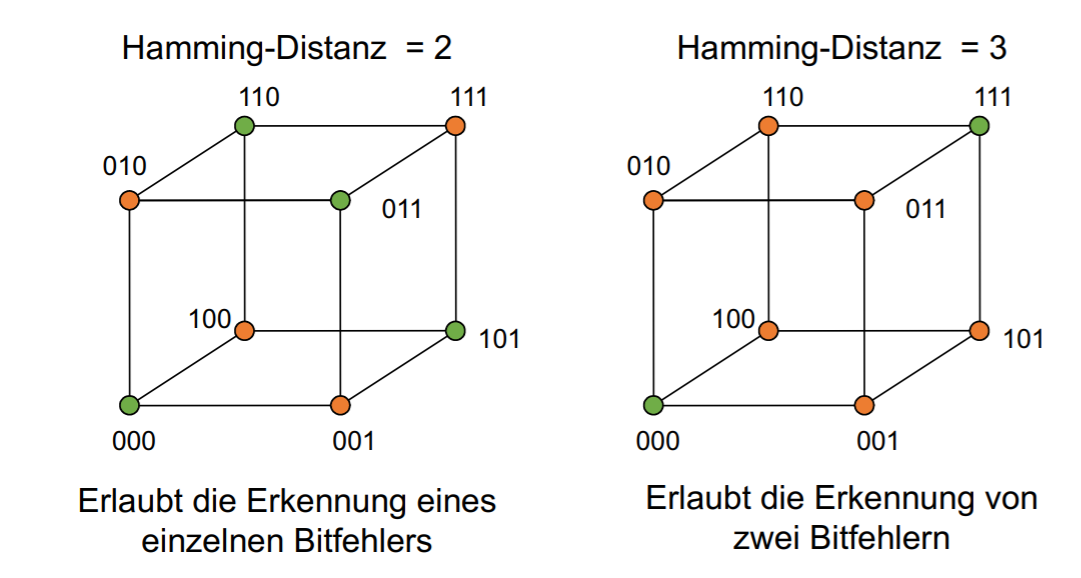
\includegraphics[width=1\linewidth]{images/hammingdist.png}
\end{center}

\subsubsection{Minimale Hamming Distanz}%
\label{ssub:minimale_hamming_distanz}

Die Hamming Distanz $d$ zwischen den Codewörtern ist nicht per se konstant.
Für eine sichere Fehlererkennung oder (später auch Fehlerkorrektur) ist
die minimale Hamming-Distanz $d_{min}(C)$ eines Codes $C$ relevant:
\[
    d_{min}(C)=min d_H (c_j, c_k)
\]

Ein \textbf{perfekter Code} liegt vor, wenn jedes empfangene Wort $w$ genau ein Codewort $c$ hat, zu dem es einen geringsten Hamming-Abstand hat und zu dem es eindeutig zugeordnet werden kann.

\subsubsection{Hamming-Gewicht}%
\label{ssub:hamming_gewicht}

Gibt an, wieviele Einsen das Codewort $c_j$ enthält. Anwendung: Bestimmung der Hamming-Distanz zweier Codewörter.
Dazu bildet man mit einer bitweisen XOR-Operation die Differenz zweier
Codewörter und bestimmt dann davon das Hamming-Gewicht, also die Anzahl
der unterschiedlichen Bits.

\subsection{Binäre Blockcodes}%
\label{sub:binäre_blockcodes}

\begin{center}
    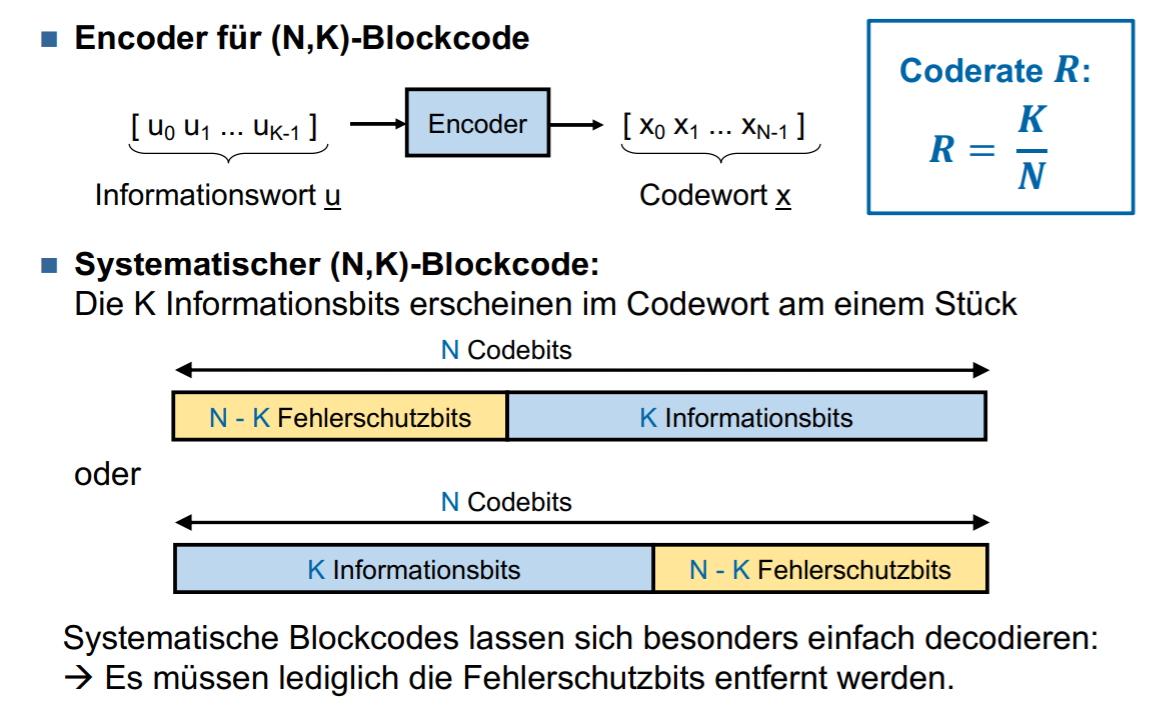
\includegraphics[width=1\linewidth]{images/blockc.png}
\end{center}

\subsubsection{Linearität}%
\label{ssub:linearität}

Bei einem \textbf{linearen (N,K) Blockcode} ist die bitweise Exor-Verknüpfung von 2 beliebigen Codewörtern (inklusive des selben) wieder ein gültiges Codewort.

Bei linearen Blockcodes ist $d_min$ das minimale Hamming-Gewicht.

\subsubsection{Zyklizität}%
\label{ssub:zyklizität}
Die zyklische Verschiebung eines Codeworts gibt wieder ein Codewort.

\subsection{Kanalcodierungstheorem}%
\label{sub:kanalcodierungstheorem}
Möchte man die Restfehlerwahrscheinlichkeit eines Fehlerschutzcodes beliebig klein machen, so muss $R < C$ sein.
\begin{enumerate}
    \item $C$: Kanalkapazität in bit/bit $C_{BSC}=1-H_b(\varepsilon)$
    \item $R$: Coderate in bit/bit $R=\frac{K}{N}$
    \item $R$ muss kleiner als $C$ sein, damit alle Informationen in den nutzbaren Bits Platz haben.
\end{enumerate}

\section{Fehlererkennung}%
\label{sec:fehlererkennung}

Jedes Codewort besteht aus $N$ Bits, wovon $K$ Informationsbits sind und $P$ Prüfbits. $N=K+P$ Mit $N$ Bits gibt es $2^N$ Möglichkeiten für Bitmuster, wovon aber nur $2^K$ gültige Codeworte sind. Die restlichen, ungültigen Bitmuster stehen zur Verfügung, um Fehler zu erkennen.

\subsection{Fehlererkennung mit Parity / Prüfsumme}%
\label{sub:fehlererkennung_mit_parity_prüfsumme}
\begin{enumerate}
    \item Even Parity: Anzahl 1er inkl. Parity-Bit ist gerade
    \item Odd Parity: Anzahl 1er inkl. Parity-Bit ist ungerade
    \item Even Parity und Odd Parity sind gleichwertig, aber nur Even Parity ist linear.
    \item Prüfsumme P = $\sum^{n-1}_{i=0}$ Element[i]
\end{enumerate}

\subsection{1-Bit Polynom-Arithmetik und CRC}%
Bei CRC werden die Bits als Koeffizienten eines Polynoms aufgefasst. \\
\textbf{Beispiel: } Das binäre Datenwort u = (101001) wird zum Polynom U(z):
\[
    U(z) = 1 \cdot z^5 + 0 \cdot z^4 + 1 \cdot z^3 + 0 \cdot z^2 + 0 \cdot z^1 + 1 \cdot z^0 = z^5 \cdot z^3 + 1
\]

Bei der Addition und Subtraktion der Koeffizienten wird die 1-Bit Arithmetik verwendet.

\begin{center}
    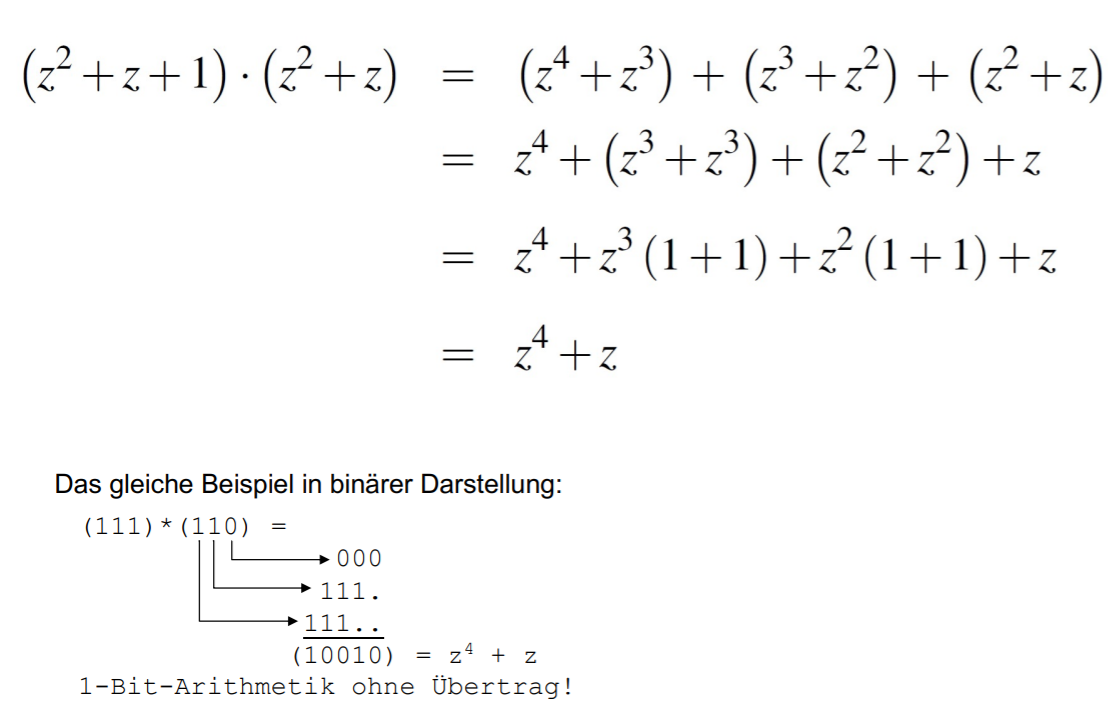
\includegraphics[width=1\linewidth]{images/crcm.png}
\end{center}

\begin{enumerate}
    \item CRC-Verfahren wird mathematisch als Modulo-2-Polynomdivision beschrieben, deren Divisionsrest die Prüfbits bildet.
    \item Generator-Polynome(Divisor) werden in der folgenden Form beschrieben: $X^4 + X + 1$, $1 \cdot X^4 + 0 \cdot X^3 + 0 \cdot X^2 + 0 \cdot X^1 + 1 \cdot X^0$ bedeutet 10011b entspricht.
    \item Der gesamte Datenbitstrom wird durch das Generator-Polynom dividiert.
    \item Der Divisionsrest wird angefügt.
    \item Die Hamming-Distanz ist nur abhängig von der Wahl des Generator Polynoms und der Länge der Daten.
\end{enumerate}

\subsubsection{CRC Encoder}%
\label{ssub:crc_encoder}

\begin{center}
    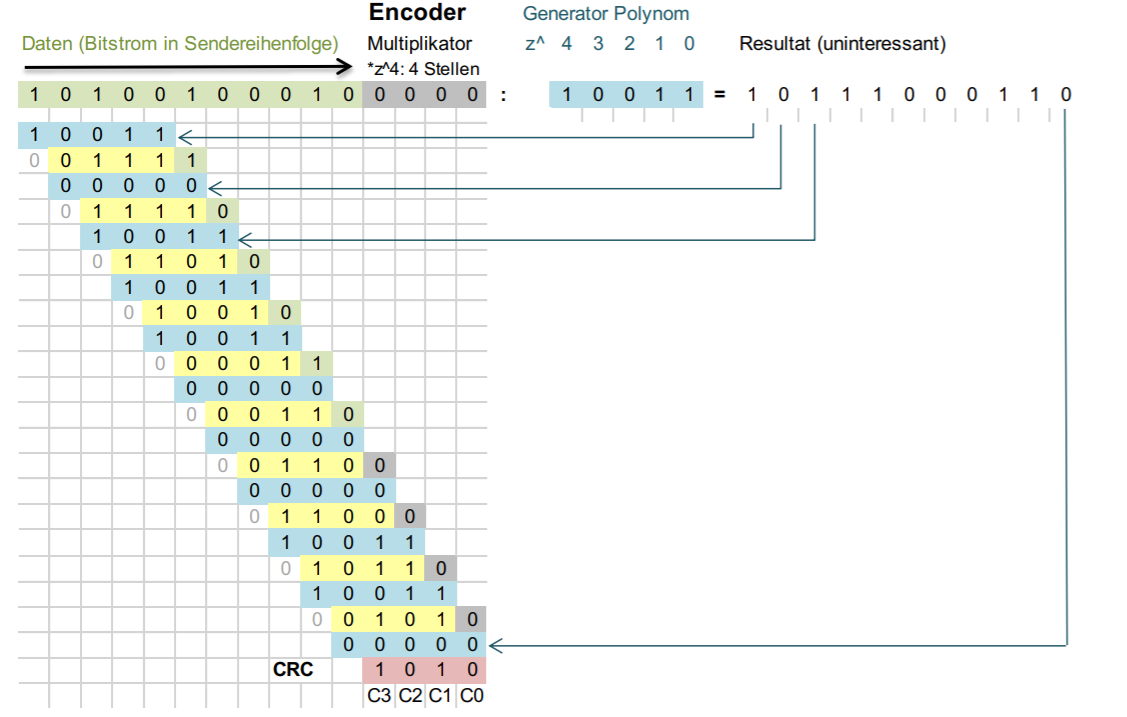
\includegraphics[width=1\linewidth]{images/crcen.png}
\end{center}

\begin{center}
    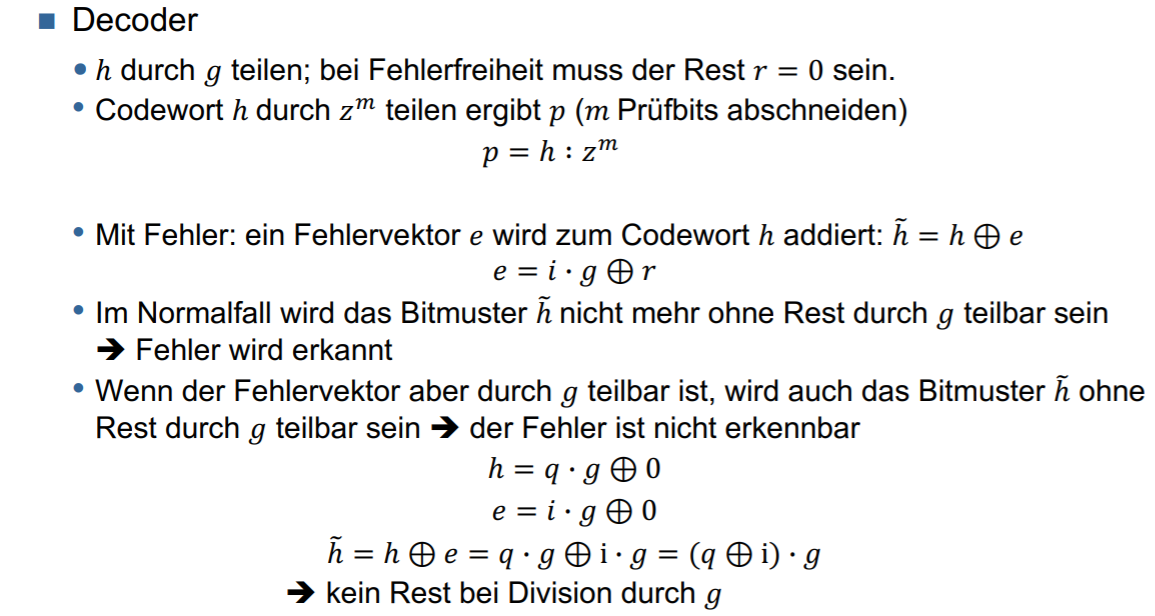
\includegraphics[width=1\linewidth]{images/crcdec.png}
\end{center}

\subsubsection{CRC Decoder}%
\label{ssub:crc_decoder}

\begin{center}
    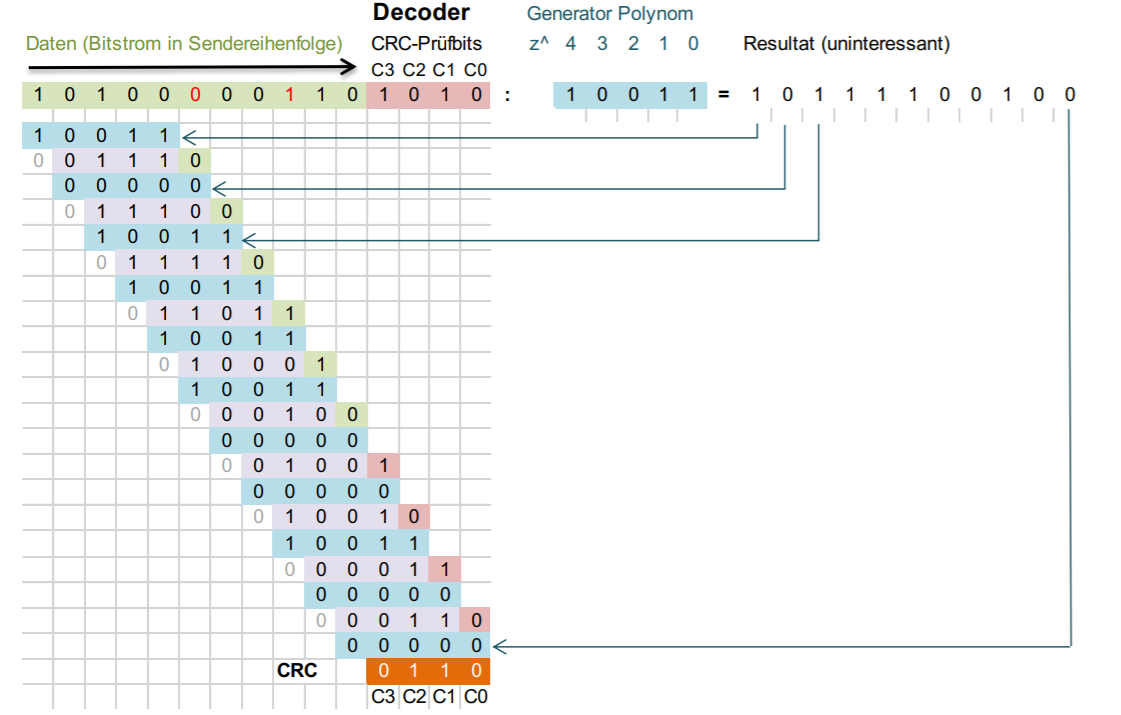
\includegraphics[width=1\linewidth]{images/crcdecp.png}
\end{center}

\subsubsection{CRC Implementierung in Hardware}%
\label{ssub:crc_implementierung_in_hardware}

\begin{center}
    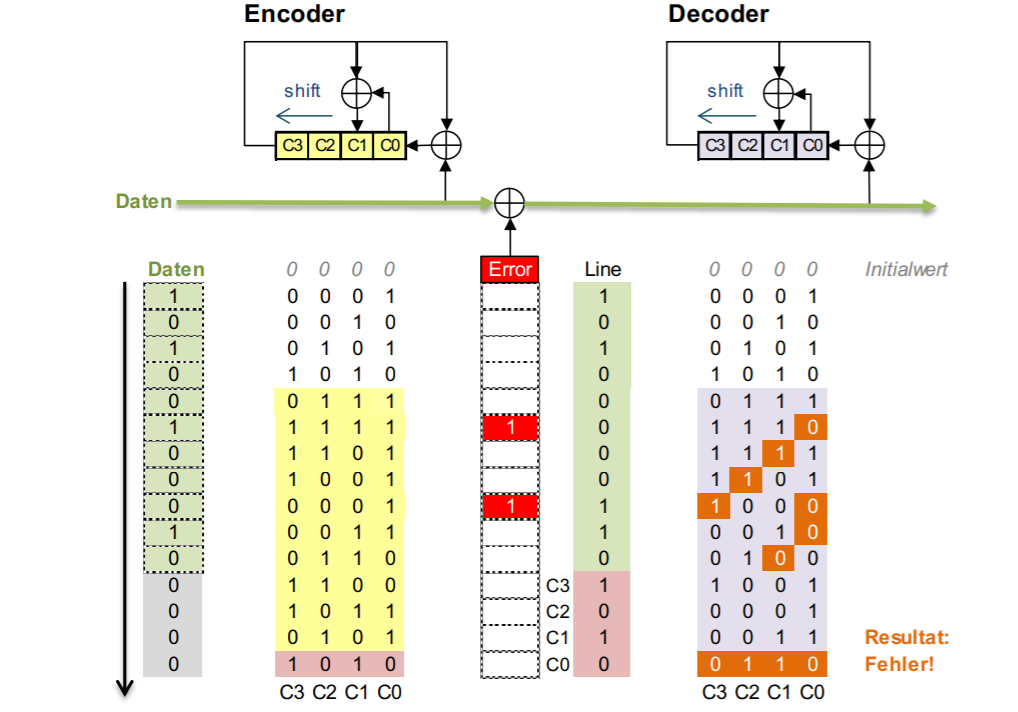
\includegraphics[width=1\linewidth]{images/crchard.png}
\end{center}

\subsubsection{CRC Polynomselektion}%
\label{ssub:crc_polynomselektion}

\begin{center}
    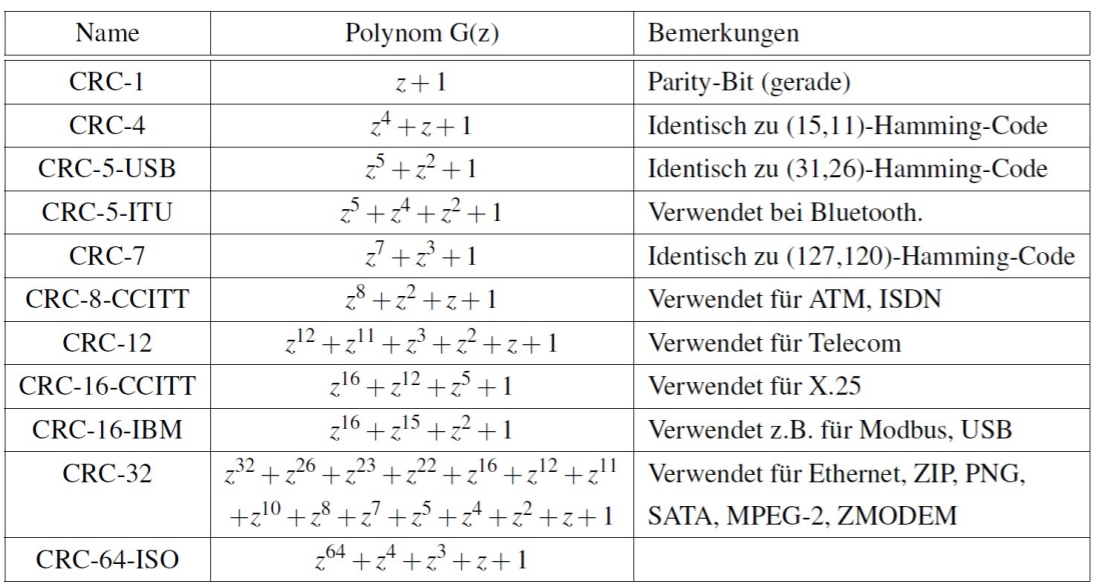
\includegraphics[width=1\linewidth]{images/crcpol.png}
\end{center}

\section{Fehlerkorrektur}%
\label{sec:fehlerkorrektur}

Die Anzahl der korrigierbaren Bitfehler (k) ist die abgerundete Hälfte der fehlerbehafteten Zwischencodes:
\[
    k \leq (d_{min} -1)/2
\]

\subsection{Blockcodes}%
\label{sub:blockcodes}

Bei Blockcodes sind bis zu $d_{min}-1$ Fehler pro Codewort erkennbar und $\frac{d_{min}-1}{2}$ Bit Fehler pro Codewort richtig korrigierbar.

\subsubsection{Prüfbits}%
\label{ssub:prüfbits}
Benötigte Prüfbits, um einen Einbitfehler in K Datenbits korrigieren zu können:
\[
    I(p) = \log_{2}(N+1), p \geq \log_2 (K + p + 1)
\]
Näherung: $I(p) \approx I(K+1) = log_2(K+1)$

\subsubsection{Hamming-Codes}%
\label{ssub:hamming_codes}
Codes mit $d_{min} = 3$ und $p = \log_2 (N+1)$ besitzen genau die minimale Anzahl benötigter Prüfbits. \\
Es sind alles perfekte Codes; für alle gilt: $d_H = d_min$ \\
Anhand von $p$ lässt sich $N$, $K$ und die Coderate $R$ berechnen:

\begin{center}
    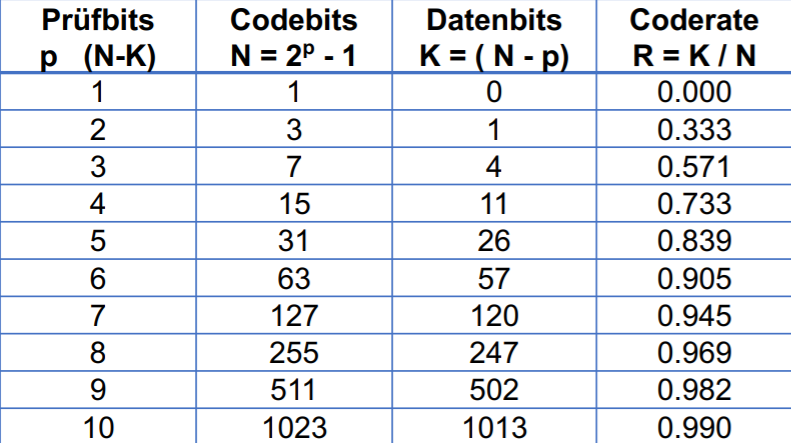
\includegraphics[width=1\linewidth]{images/hammingcodes.png}
\end{center}

\subsubsection{Lineare Blockcodes - Encoder}%
\label{ssub:lineare_blockcodes}
Hamming-Codes gehören zu den linearen (N,K) Blockcodes. Sie werden durch eine Generatormatrix definiert, die sich aus einer Paritätsmatrix und einer Einheitsmatrix zusammensetzt.

\begin{center}
    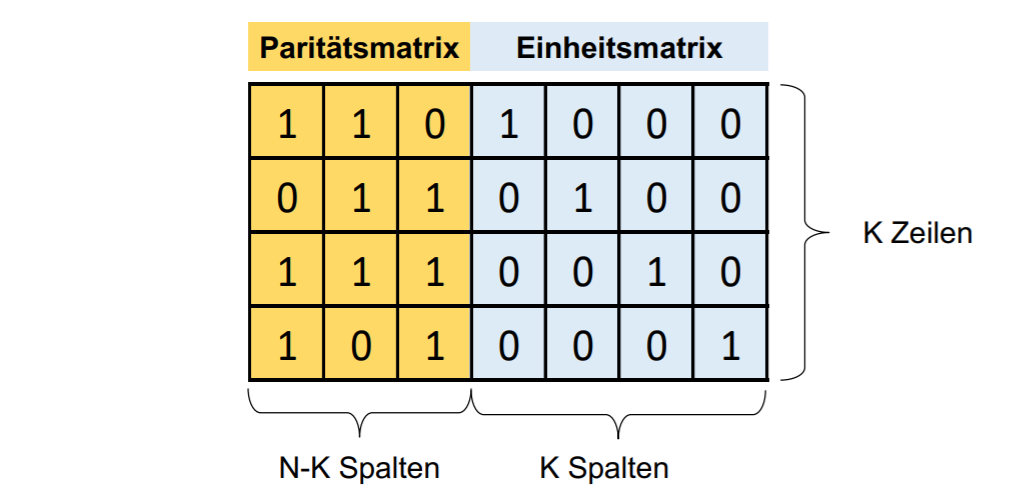
\includegraphics[width=1\linewidth]{images/linearbl.png}
\end{center}

Beispiel mit einem (7,4) Hamming-Code:
\[
    \begin{pmatrix}
    1 & 1 & 0 & 1 & 0 & 0 & 0 \\
    0 & 1 & 1 & 0 & 1 & 0 & 0 \\
    1 & 1 & 1 & 0 & 0 & 1 & 0 \\
    1 & 0 & 1 & 0 & 0 & 0 & 1 
    \end{pmatrix}
\]
Das Nutzdatenwort $u_{10} = (1010)$ wird mit der Matrix multipliziert, wodurch das Codewort $0011010$ entsteht. \\
Die Generatormatrix nimmt also Nutzdatenvektoren der Länge $K=4$ auf und produziert daraus Codeworte der Länge $N=7$. \\
Jedes Codewort $c_j$ ist eine Linearkombination von Zeilen der Generatormatrix $G_h$ ist. \\
Die rechten vier Spalten der Generatormatrix $G_h$ bilden eine Einheitsmatrix $I^{4x4}$. Diese Einheitsmatrix bewirkt, dass an der betreffenden Stelle im Codewort $c_j$, also rechtsbündig, der Nutzdatenvektor $u_j$ erscheint. Ein Code mit einer derartigen Generatormatrix ist demnach systematisch und lässt sich besonders leicht decodieren.
\vfill
\subsubsection{Lineare Blockcodes - Decoder}%
\label{ssub:lineare_blockcodes_decoder}

Aus der Generatormatrix wird eine Prüfmatrix gebildet. Schliesslich wird das empfangene Bitmuster mit dieser multipliziert und anschliessend das Syndrom bestimmt.
\[
    s = \underline{\tilde{x}} \cdot \underline{H}^T = (\underline{c}_j + \underline{e}) \cdot \underline{H}^T=\overbrace{\underline{c}_j \cdot \underline{H}^T}^{\text{=0}}+\underline{e} \cdot \underline{H}^T=\underline{e} \cdot \underline{H}^T
\]

Jedes gültige Codewort $\underline{c}_j$ multipliziert mit der Prüfmatrix $\underline{H}^T$ ergibt $0$. Das Symbol ist also gleich dem Produkt von Fehlervektor und Paritätsprüfmatrix.\\

\subsubsection{Bildung der Generatormatrix und Prüfmatrix}%
\label{ssub:bildung_der_generatormatrix}

\begin{enumerate}
    \item Die Generatormatrix setzt sich aus einer Paritätsmatrix und einer Einheitsmatrix zusammen.
    \item Die Paritätsbits müssen voneinander unabhängig sein; jede Spalte muss unterschiedlich sein.
    \item Der Code ist linear. Für die geforderte $d_{min} = 3$ muss jeder Code (ausser dem Null-Code) mindestens 3 Einsen enthalten.
\end{enumerate}

\begin{center}
    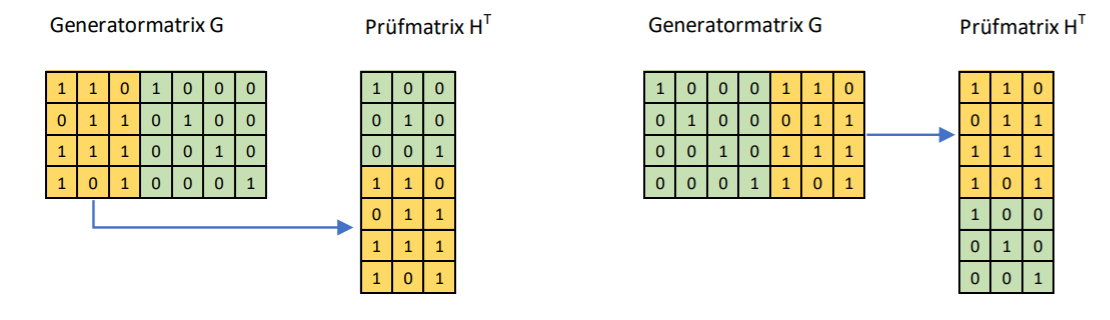
\includegraphics[width=1\linewidth]{images/preufmatrix.png}
\end{center}

\begin{center}
    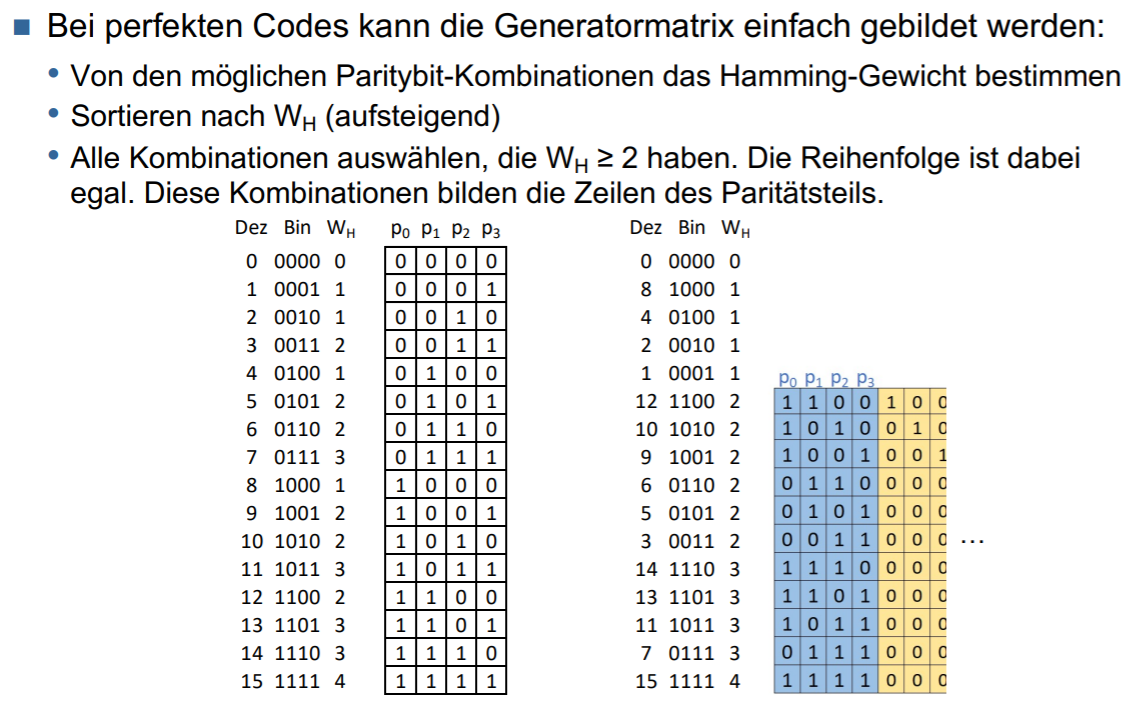
\includegraphics[width=1\linewidth]{images/bilgen.png}
\end{center}

\subsubsection{Blockcode dekodieren - Verfahren}%
\label{ssub:blockcode_dekodieren_verfahren}

\begin{enumerate}
    \item Berechnung des Syndroms: $\underline{s}=\underline{\tilde{c}} \cdot \underline{H}_h^T$
    \item Syndrom bzw. Fehler Tabelle erstellen (Wie bei Codeworten, jede zeile der matrix ist jeweils ein syndrom)
    \item Fehlerkorrektur (Fehlervektor aus Tabelle mit Fehlerhaftem Code addieren): $\hat{c} = \underline{\tilde{c}} + \underline{\hat{e}}$
    \item Decodierung: $\underline{\hat{c}} \implies \underline{\hat{u}}$
\end{enumerate}

\section{Faltungscodes}%
\label{sec:faltungscodes}
\subsection{Zustandsdiagramm}%
\label{sub:zustandsdiagramm}

\begin{center}
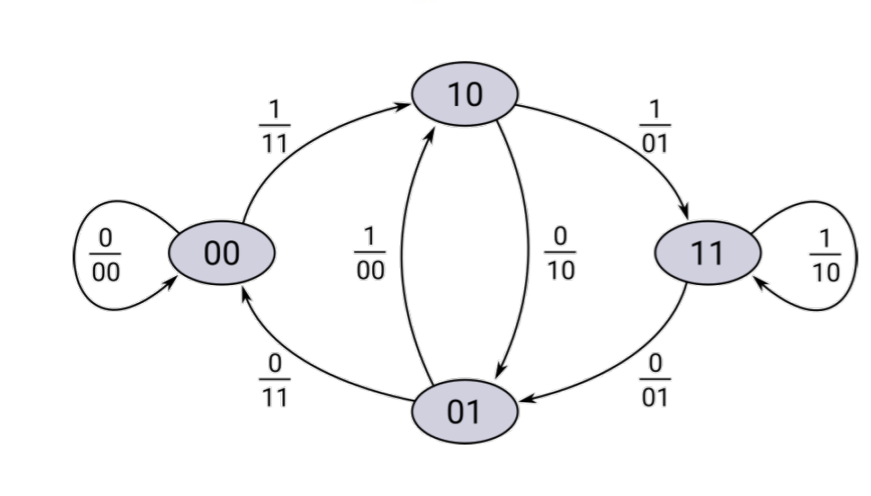
\includegraphics[width=1\linewidth]{images/zstfal.png}
\end{center}

\subsection{Hardware Implementierung}%
\label{sub:hardware_im}

\begin{center}
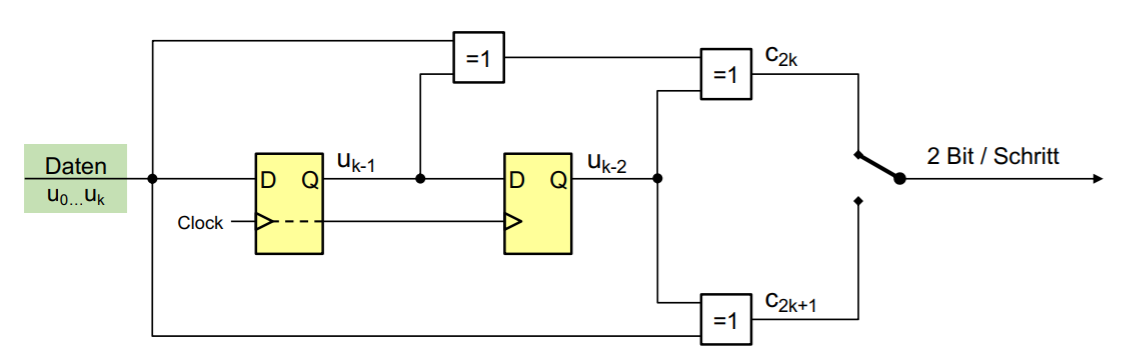
\includegraphics[width=1\linewidth]{images/falthard.png}
\end{center}

\subsection{Freie Distanz}%
\label{sub:freie_distanz}
Bei Faltungscodes spricht man nicht von minmaler Hamming-Distanz, sondern von $d_{free}$ freier Distanz.\\
Da Faltungscodes stets linear sind, gilt auch $d_{free}=w_{min}$. \\

\subsubsection{Anzahl korrigierbarer Fehler}%
\label{ssub:anzahl_korrigierbarer_fehler}
\[
    \frac{d_{free}-1}{2}, N=3 ... 6 \cdot m \text{Bits}
\]

\subsubsection{Optimum free Distance}%
\label{ssub:optimum_free_distance}

\begin{enumerate}
    \item $\gamma$ bezeichnet die Anzahl Generatoren, $m$ die Länge des Schieberegisters resp. die Anzahl zustände des Encoders
    \item Es zeigt sich, dass zu jedem Wertepaar $(\gamma; m)$ eine maximal mögliche freie Distanz gibt.
    \item Codes, die diese freie Distanz erreichen, nennt man Optimum Free Distance Codes.
\end{enumerate}

\begin{center}
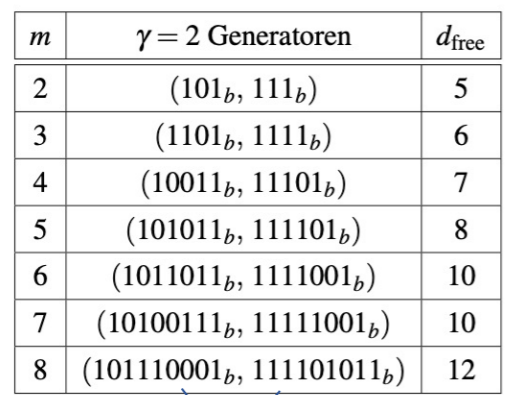
\includegraphics[width=1\linewidth]{images/ofdcodes.png}
\end{center}

\subsection{Viterbi Decoder}%
\label{sub:viterbi_decoder}

\begin{center}
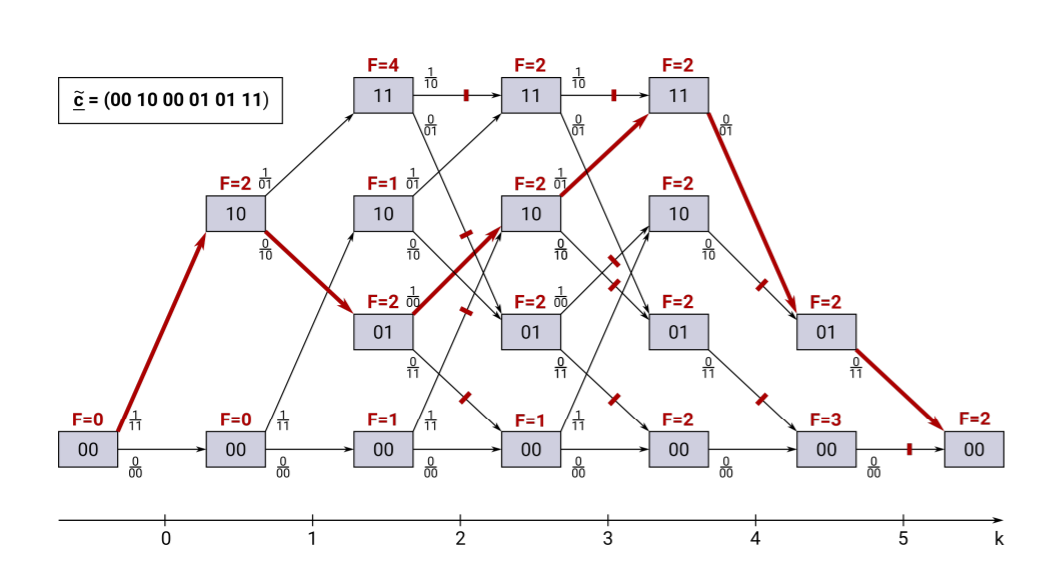
\includegraphics[width=1\linewidth]{images/trellis.png}
\end{center}

\begin{enumerate}
    \item Initialisierung: Am Anfang befindet man sich im Startzustand (00) und initialisiert dessen Fehlerwert zu $F=0$
    \item Bei $k=0$ gibt es zwei mögliche Übergänge vom Startzustand aus:
        \begin{itemize}
            \item Bei Eingangsbit $u_0$ = 0 gib es einen Übergang zum Zustand (00). Man vergleicht die Ausgangsbits im Trellis (hier 00) mit den ersten beiden Bits im Bitmuster und notiert die Fehler.
            \item Bei Eingangsbit = 1 findet ein Zustandswechsel zu (10) statt. Auch hier vergleicht man wieder die Ausgangsbits (11) mit den Eingangsbits im Trellis mit den ersten beiden Bits im Bitmuster und notiert die Fehler
        \end{itemize}
    \item Dies wird so weitergeführt für jede Abzweigung. Wenn mehrere Übergänge zu einem Zielzustand führen nimmt man jeweils den mit den wenigsten Bitfehlern. Die Fehler werden dabei laufend addiert! Wenn bei einer Abzweigung ein Fehler von 1 besteht und bei der nächsten ein Fehler von 2, dann notiert man eine 3 und nicht eine zwei.
    \item Um schliesslich die Schätzung für das ursprüngliche Codewort zu finden, läuft man vom Endzustand rückwärts durch den Trellis bis zum Anfang. Dabei nimmt man immer den Weg mit den wenigsten Fehlern.
    \item Schliesslich findet man den Vektor, mit dem man dann von Vorne den Pfad nochmals verfolgen und schliesslich das ursprüngliche Wort herausfinden kann (Tail-Bits beachten).
\end{enumerate}

